\chapter{感知机代码仿真}

\section{算法描述}

代码实现思路为:初始化权重,如果实例点正确分类,则检查下一个实例点,指标指向下一个实例点,
如果实例点被误分类,则更新权重,指标回到第一个检查的实例点重新开始检查,直到找到权重使得
从第一个到最后一个实例点都被正确分类。

\begin{lstlisting}[language=Python]
import numpy as np
import matplotlib.pyplot as plt

# 定义感知机模型类
class Perceptorn:
    def __init__(self):
        self.count = 1
        self.w = None
        self.b = 0
        self.l_late = 1
    
    def fig(self):
        # 模型方程
        x_plot = np.linspace(2, 7,10)
        y_plot = -(perceptorn.w[0]*x_plot+perceptorn.b)/perceptorn.w[1]
        # 图示
        plt.plot(x_plot,y_plot)
        plt.scatter(x_trian[0:3,0],x_trian[0:3,1],marker='+', color='orange',label='postive')
        plt.scatter(x_trian[3:6,0],x_trian[3:6,1],marker='+', color='green',label='negtive')

        #设置图例
        plt.legend(loc=1)

        #显示
        plt.show()

    # 算法主函数
    def fit(self,x_trian,y_trian):
        cnt=0
        self.w=np.zeros(x_trian.shape[1])#shape 方法通常用于获取数组或矩阵的形状(维度),主要用于 NumPy 库中的数组对象。
        i = 0

        while i < x_trian.shape[0]:
            x = x_trian[i]
            y = y_trian[i]
            # 判断其所有点是否都没有误分类,如有更新w,b,重新判断
            if y*(np.dot(self.w,x)+self.b)<=0:
                self.w = self.w + self.l_late*np.dot(x,y)
                self.b = self.b+self.l_late*y
                i = 0
            else:
                i += 1
                
            cnt=cnt+1
    
        print("trainning finish ! trainning cost times : {}".format(cnt))
            
\end{lstlisting}

利用感知机模型,对下列的测试数据进行训练

\begin{lstlisting}[language=Python]
# 训练集
x_trian = np.array([[3,3],[3,5],[4,7],[4,0],[2,1],[6,2]])
y_trian = np.array([1,1,1,-1,-1,-1])
print(x_trian.size,y_trian.size)
\end{lstlisting}

调用Perceptron类对数据进行训练,得到结果如下

\begin{figure}[H]
    \centering
    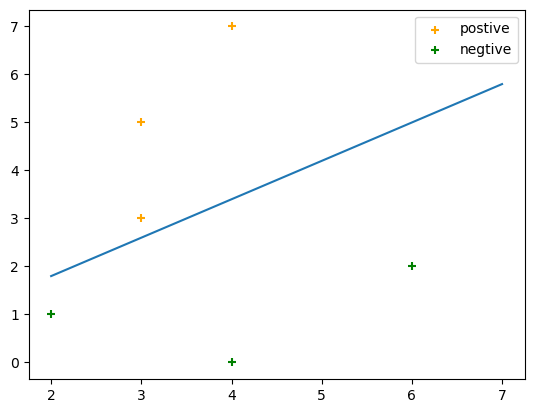
\includegraphics[scale=0.5]{figures/perceptron1.png}
    \caption{训练成果}
\end{figure}

算法的训练次数为21次,权重向量为$[-4.  5.]$,偏置为 $-1$。

\section{实战}

下面的例子是$sklearn$里面的鸢尾花的例子。首先导入需要的包和数据集。

\begin{lstlisting}[language=Python]
import pandas as pd
import numpy as np
from sklearn.datasets import load_iris
from sklearn.linear_model import Perceptron
import matplotlib.pyplot as plt
\end{lstlisting}


加载数据集,并且把数据集转换为Dataframe类型。
\begin{lstlisting}[language=Python]
# 处理数据
iris = load_iris()
data = pd.DataFrame(iris.data,columns=iris.feature_names)
\end{lstlisting}

DataFrame 是 pandas 中最重要的数据结构之一,类似于 Excel 表格或 SQL 表。DataFrame 可以包含
多种类型的数据,包括整数、浮点数、字符串等,并且可以轻松地进行数据操作和分析。

鸢尾花的数据表格如下所示

\begin{figure}[H]
    \centering
    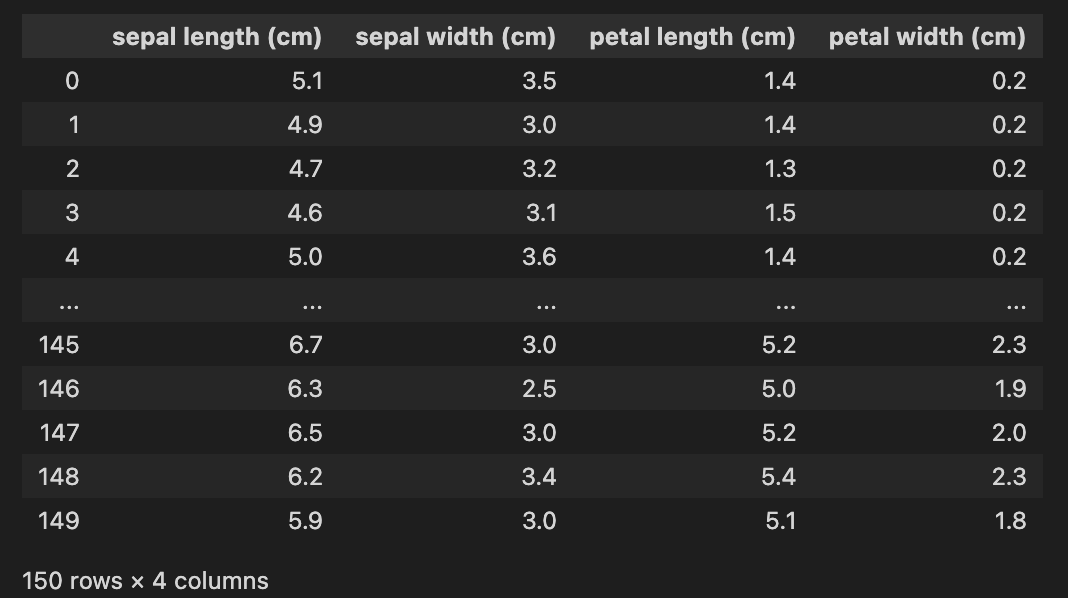
\includegraphics[scale=0.4]{figures/鸢尾花数据集.png}
    \caption{鸢尾花数据集}
\end{figure}

其中分为花萼的长宽和花瓣的长宽,接下来加载标签值。

\begin{lstlisting}[language=Python]
data['label'] = iris.target #标签值
data.columns = ['sepal length', 'sepal width', 'petal length', 'petal width', 'label']
print(data.head(4))
\end{lstlisting}

标签值如下

\begin{figure}[H]
    \centering
    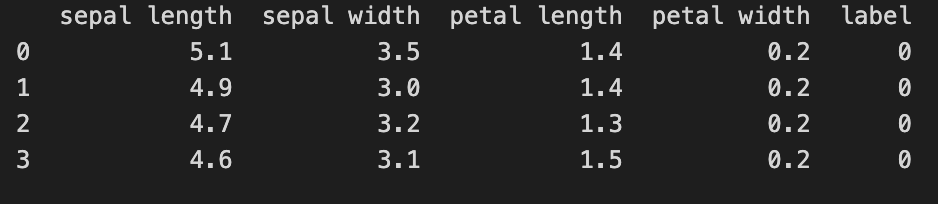
\includegraphics[scale=0.4]{figures/鸢尾花标签值.png}
    \caption{鸢尾花数据集}
\end{figure}

我们用花萼的数据来训练模型,可视化数据集图像如下

\begin{figure}[H]
    \centering
    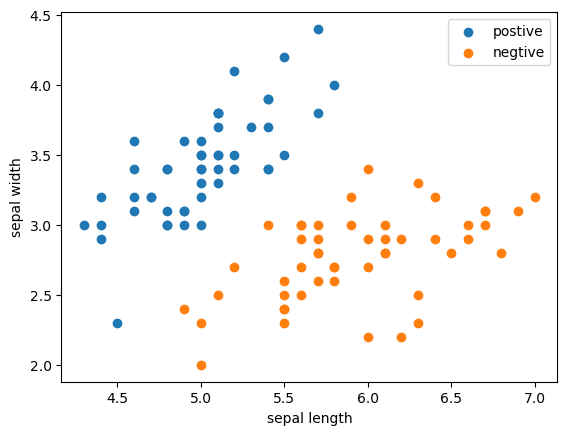
\includegraphics[scale=0.6]{figures/鸢尾花花萼图像.png}
    \caption{鸢尾花数据集的二维分布}
\end{figure}

可以直观地看出,数据集明显是线性可分的。我们例化sklearn中的感知机模型,代码如下
\begin{lstlisting}[language=Python]
x_train = np.array(data.iloc[:100,[0,1]])
y_train = np.array(data.iloc[:100,-1])

perceptron = Perceptron()
perceptron.fit(x_train,y_train)
print('w:',perceptron.coef_,'\n','b:',perceptron.intercept_,'\n','迭代次数:',perceptron.n_iter_)
    
# 评判模型
res = perceptron.score(x_train, y_train)
print('成功率:{:.0%}'.format(res))
\end{lstlisting}

拟合次数为8次,得到的拟合超平面如下
\begin{figure}[H]
    \centering
    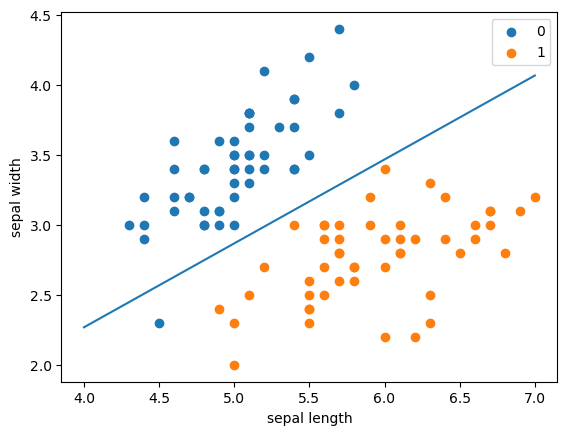
\includegraphics[scale=0.6]{figures/鸢尾花数据拟合超平面.png}
    \caption{鸢尾花数据集的二维分布}
\end{figure}

可见拟合结果中有一个被误分类,但是总体上是成功分类了。